\chapter{PGF in C++}
\lettrine[lines=4, loversize=-0.1, lraise=0.1]{T}{his chapter describes} the C++ library for reading pgf files and using the contained grammar to parse and linearise text. It is based largely on the existing Java library JPGF that is used in the Android application.


\section{libpgf}
There already exists a C library to work with PGF files \cite{libpgf}. However, it does not support predicting the next possible tokens given a sequence of previous tokens. As this was a rather prominent feature of the Android aplication, not providing it in the iPhone application was not an alternative which meant that this existing library unfortunately could not be used.


\section{JPGF}
The Android application uses the JPGF library \cite{jpgf}. It uses ... to parse the input and is thus able to predict possible continuations of the current token sequence.

The JPGF library is divided into four major parts: The PGF file reader, the lineariser, the parser, and finally the parse tree represenatation. These will be discussed further in the next section.


\section{libpgf+}
The C++ library retains most of the structure and api of the Java library. Some additions were necesarry to account for the fact that C++ does not provide garbage collection, automatic reference counting or any other form of automatic memory management except on the stack \cite{cppmemoryhandling}. Also, some changes were made in cases where there were duplicate methods with different names or where methods did not follow the general naming convention used in JPGF.


\subsection{Memory handling}
As C++ does not provide automatic memory management and JPGF relies on the garbage collector in Java taking care of all allocated objects that it no longer needs, something was needed to take care of this in the new implementation. There were some alternatives. One was to implement reference counting \cite{refcount} in the api. Another alternative would have been to implement garbage collection (GC) \cite{gc} or rely on an external library to provide it. A comparison of the three alternatives can be seen in table \ref{tbl:memorymanagement}.

\begin{table}
\begin{tabularx}{\textwidth}{|l|X|X|}
	\hline
	 & \emph{Pros} & \emph{Cons} \\ \hline
	\emph{Reference counting} & No external dependencies. Easy to implement. & Requires the programmer to always release acquired references by hand. \\ \hline
	\emph{Internal GC} & No external dependencies. Easy to use, the programmer does not need to do any manual release of references when they are no longer needed. & Very large project to implement. Outside the scope of this thesis. \\ \hline
	\emph{External GC} & Easy to use, the programmer does not need to do any manual release of references when they are no longer needed. & Adds external dependencies to the library. \\ \hline
\end{tabularx}
\caption{Comparison of memory management alternatives.}
\label{tbl:memorymanagement}
\end{table}

From these three alternatives, reference counting was chosen. The implementation uses a base class which provides methods for counting references that is then inherited either directly or indirectly by all other classes in the library. The interface for the reference counting class can be seen in listing \ref{lst:refbase}.

\lstinputlisting[language=C++, frame=single, breaklines=true, float, captionpos=b, linerange={16-26,30-32}, caption=Base class for all reference counted classes., label=lst:refbase]{../pgf+/include/gf/RefBase.h}

The reference counting implementation also provides a convenience function to simultaenously release a reference and clear the pointer to prevent lingering references. This function can be seen in listing \ref{lst:release}.

\lstinputlisting[language=C++, frame=single, breaklines=true, float, captionpos=b, linerange={34-39}, caption=Convenience method to release and clear references., label=lst:release]{../pgf+/include/gf/RefBase.h}


\subsection{Exceptions}
There are a number of different things that can go wrong when handling a grammar. First of all, it might not be possible to read it from the PGF file for some reason. Other failures may arise in the parser or lineariser. JPGF indicates these failures with Java exceptions, which can fairly easy be translated to C++ exceptions.

To further simplify this, all exceptions thrown by the library were given a common base class shown in listing \ref{lst:exception}. Unlike most other classes in the library, this does not inherit from the reference counting base class. The reason for this is how C++ exception handling works. When an exception is thrown it is first constructed on the stack, and then copied into a buffer provided by the system. This buffer is then the responsibility of the system and will be automatically deallocated once the exception has been caught.

\lstinputlisting[language=C++, frame=single, breaklines=true, float, captionpos=b, linerange={17-31}, caption=Base class for all exceptions thrown in the library., label=lst:exception]{../pgf+/include/gf/Exception.h}


\subsection{PGF}
This is the main class representing the grammar loaded from a PGF file. The interfaces is almost identical to the corresponding class in JPGF and can be seen in listing \ref{lst:pgfclass}. It provides methods to retrieve the abstract syntax of the grammar, to retrieve any of the concrete syntaxes available in the grammar and also to enumerate all of them. In addition it provides methods for getting the version information of the PGF file that it represents.

\lstinputlisting[language=C++, frame=single, breaklines=true, float, captionpos=b, linerange={25-25,33-33,47-47,55-55,61-61,67-67,73-73,81-81,87-88}, caption=Main class representing the grammar., label=lst:pgfclass]{../pgf+/include/gf/PGF.h}


\subsection{Reader}
The reader consists of two parts. The first part is the PGFReader class that does the actual parsing of the PGF file. Its public api can be seen in listing \ref{lst:pgfreader}. It consists only of two constructors and a method to read the PGF file and create a PGF object. Both constructors take a c stream as argument that will be used when reading the file. The second constructor also accepts a set of language names that will be used to filter which concrete syntaxes are loaded from the file.

\lstinputlisting[language=C++, frame=single, breaklines=true, float, captionpos=b, linerange={42-42,347-349,358-359}, caption=Base class for all exceptions thrown in the library., label=lst:pgfreader]{../pgf+/include/gf/PGFReader.h}

The second part is the set of classes modelling the grammar that was read from the file. There are classes corresponding to each type described in section \ref{sec:pgf}. The model is the same as the one used in JPGF and can be seen in figure \ref{fig:grammarmodel}.

\begin{figure}[htb]
\centering
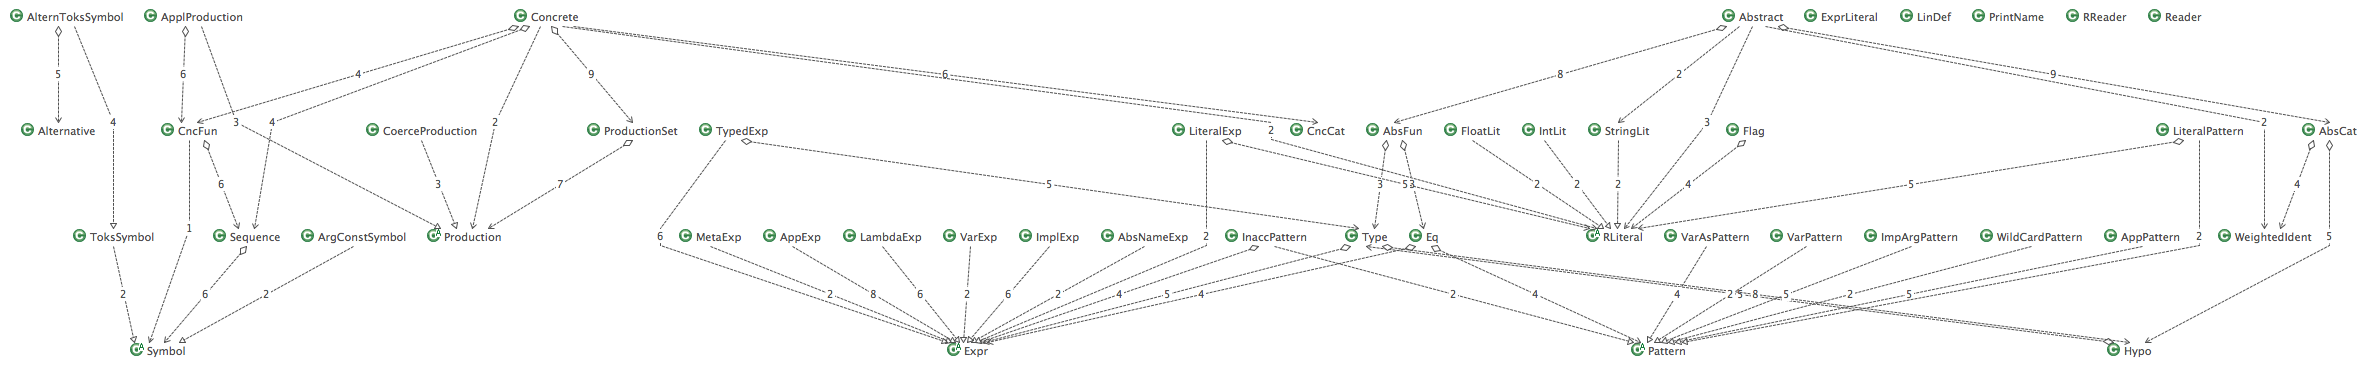
\includegraphics[width=\textheight,angle=90]{fig/grammarmodel}
\caption{Class diagram of the grammar model.}
\label{fig:grammarmodel}
\end{figure}


\subsection{Parse tree}
The classes modelling the parse tree are automatically generated from the BNF grammar shown in listing \ref{lst:parsetree} using bnfc \cite{bnfc}. This grammar is identical to the one used in JPGF and theoretically a tree parsed with libpgf+ could be converted to a string using this grammar and then read from the string with JPGF and linearised there, or vice versa.

\lstinputlisting[language=Haskell, morekeywords={Ident}, frame=single, breaklines=true, float, captionpos=b, caption=BNF grammar used to generate the classes modelling the parse tree., label=lst:parsetree]{../pgf+/src/Trees.cf}

\subsection{Lineariser}
\subsection{Parser}
